% !TeX encoding = UTF-8
% !TeX program = xelatex

\documentclass{YNUbachelor}
\usepackage{myPackages}

\title{云南大学本科学生毕业论文(设计)\;\LaTeX 模板}
\school{XX学院}
\author{XXX}
\studentID{20181050000}
\major{XX学}
\teacher{XXX}

\begin{document}
	
	\cover
	
	\copyrightpage
	
	\maketitle

	\toc

	\begin{abstract}
		中文摘要
	\end{abstract}

	\keywords{关键词1;关键词2;关键词3}

	\begin{enabstract}
		English Abstract
	\end{enabstract}

	\enkeywords{enKeyWords1;enKeyWords2;enKeyWords3}
		
	\section{基本使用说明}
		声明:\href{https://gitee.com/Astro-Lee/YNU-thesis-bachelor}{云南大学本科毕业论文(设计) LaTeX 模板}根据\href{http://www.jwc.ynu.edu.cn/info/1003/2052.htm}{《云南大学本科学生毕业论文(设计)工作要求及规范》}编写,个人能力、精力有限,不保证完全符合规范!此外,该模板未经学校官方核准,如有顾虑,请不要使用!
		
		对于第一次使用\LaTeX 的同学推荐先阅读\href{http://mirrors.ctan.org/info/lshort/chinese/lshort-zh-cn.pdf}{一份(不太)简短的 \LaTeXe 介绍}。
		
		\subsection{编码及编译要求}
		\lstinline[language=latex]|main.tex|源代码必须保存为UTF-8编码,并使用XeLaTeX编译器进行编译,其在源代码应中对的语句为:
		
	\begin{latexcode}
		% !TeX encoding = UTF-8
		% !TeX program = xelatex
	\end{latexcode}
		
		注意:在\LaTeX 源代码中``\lstinline[language=latex]|%|''是注释符,但以上代码会指定相应的设置,因此在设置正确的前提下才能将其删去。要学会使用注释符,当你知道注释哪部分内容会编译得什么效果时,那你已经具备了用\LaTeX 撰写文档的基本能力。这也是我把《用户使用手册》写进此模板中的原因。另外,符号``\lstinline[language=latex]|\|''可以调用宏命令,形如\lstinline[language=latex]|\命令名[<可选参数>]{<必选参数>}|,也可以开启一个环境,形如\lstinline[language=latex]|\begin{<环境名>}[<可选参数>] ... \end{<环境名>}|,它还是一个转义符。这里使用符号\lstinline[language=latex]|< >|表示选项。
		
	\subsection{文档类和所需的宏包}
		通过如下命令导入文档类和所需的宏包:
	\begin{latexcode}
		\documentclass{YNUbachelor}
		\usepackage{myPackages}
	\end{latexcode}

	注意:为了使\lstinline[language=latex]|main.tex|源代码更加简洁,建议在\lstinline[language=latex]|myPackages.sty|文件中添加所需的宏包。
		
		\subsection{论文信息}
		将论文信息填在如下命令中:
	\begin{latexcode}
		\title{云南大学本科学生毕业论文(设计)\;\LaTeX 模板}
		\school{XX学院}
		\author{XXX}
		\studentID{20181050000}
		\major{XX学}
		\teacher{XXX}
	\end{latexcode}

	强烈建议将以上的这些代码写在\lstinline[language=latex]|main.tex|源代码靠前的位置。
	
	\section{撰写论文}
	\subsection{document环境}
	\lstinline[language=latex]|main.tex|文件中有且仅有一个\lstinline[language=latex]|document|环境,{\color{red}\bfseries 在此之后的所有代码}都必须写在\lstinline[language=latex]|document|环境中。
	\begin{latexcode}
		\begin{document}
			%此后的所有代码都必须写在这里
		\end{document}
	\end{latexcode}
	
	\subsection{论文封面、声明页、标题和目录}
	使用如下代码插入论文的封面、声明页、标题和目录:
	\begin{latexcode}
		\cover%论文封面
		
		\copyrightpage%声明页
		
		\maketitle%论文标题
		
		\toc%目录
	\end{latexcode}

	\subsection{中英文摘要及关键词}
	使用如下代码插入中英文摘要及关键词:
	\begin{latexcode}
		\begin{abstract}
			中文摘要
		\end{abstract}
		
		\keywords{关键词1;关键词2;关键词3}
		
		\begin{enabstract}
			English Abstract
		\end{enabstract}
		
		\enkeywords{enKeyWords1;enKeyWords2;enKeyWords3}
	\end{latexcode}
	
	\subsection{章节标题和段落}
	
	本模板中,一级标题、二级标题和三级标题分别使用\lstinline[language=latex]|\section{<一级标题名>}|、\lstinline[language=latex]|\subsection{<二级标题名>}|和\lstinline[language=latex]|\subsubsection{<三级标题名>}|表示。{\color{red}\bfseries 分段应空一行},换句话说:分段应按两次回车键,而不是一次。例如:
	
	\begin{latexcode}
		\section{一级标题名}
		这是第一段。
		
		这是第二段。
			\subsection{二级标题名}
			这是第一段。
			
			这是第二段。
				\subsubsection{三级标题名}
				这是第一段。
				
				这是第二段。
	\end{latexcode}
	
	\subsection{数学环境}
	
	在论文中排版数学符号、行内公式和行间公式是很方便的。对于初学者,推荐使用\href{https://www.latexlive.com/}{在线\LaTeX 公式编辑器}来辅助编辑\LaTeX 公式。以下介绍行内公式和行间公式的排版方式:
	\subsubsection{行内公式}
		行内公式应使用\lstinline[language=latex]|$ <公式的代码> $|来表示。例如:
	\begin{latexcode}
		勾股定理$a^2+b^2=c^2$。
	\end{latexcode}\textbf{编译得:}勾股定理$a^2+b^2=c^2$。

	\subsubsection{行间公式}
		行间公式应使用\lstinline[language=latex]|\[ <公式的代码> \]|来表示。例如:
	\begin{latexcode}
		勾股定理:
		\[
			a^2+b^2=c^2
		\]
	\end{latexcode}\textbf{编译得:}勾股定理:\[a^2+b^2=c^2\]
	
	\subsubsection{带有编号的行间公式}
		带有编号的行间公式应使用\lstinline[language=latex]|align|等环境来表示。例如:
		
	\begin{latexcode}
		勾股定理:
		\begin{align}
			a^2+b^2=c^2\label{eq:Pythagoras theorem}
		\end{align}
	\end{latexcode}
	\textbf{编译得:}勾股定理:\begin{align}
	a^2+b^2=c^2\label{eq:Pythagoras theorem}
	\end{align}

	\subsubsection{带编号公式的引用}
	上一小节中的\lstinline[language=latex]|\label{eq:Pythagoras theorem}|给公式一个标签,方便交叉引用。例如:
	
	\begin{latexcode}
		引用勾股定理,\autoref{eq:Pythagoras theorem}。
	\end{latexcode}\textbf{编译得:}引用勾股定理,\autoref{eq:Pythagoras theorem}。

	可以交叉引用的还有图片、表格和章节等,使用的方式相同。推荐一个在线的符号识别网站\href{http://detexify.kirelabs.org/classify.html}{Detexify}。

	\subsection{插图}
	\subsubsection{插入图片的一般方式}
	在论文中,插入图片或表格一般使用浮动体环境。\LaTeX 预定义了\lstinline[language=latex]|figure|和\lstinline[language=latex]|table|两类浮动体环境,通常为\lstinline[language=latex]|figure|里放图片,\lstinline[language=latex]|table|里放表格。这里以\lstinline[language=latex]|figure|环境为例,代码如下:
	
	\begin{latexcode}
		\begin{figure}[<允许位置>]
			...
		\end{figure}
	\end{latexcode}\lstinline[language=latex]|<允许位置>|参数用来设定浮动体排版的位置,通常有\lstinline[language=latex]|h|、\lstinline[language=latex]|t|、\lstinline[language=latex]|b|、\lstinline[language=latex]|p|、\lstinline[language=latex]|!|及其组合。常用组合选项为\lstinline[language=latex]|htbp|,其表示图片放置优先级为:当前位置>页面顶部>页面底部>放置在允许有浮动对象的页面上。

	使用本文档类已调用的\lstinline[language=latex]|float|宏包提供的\lstinline[language=latex]|H|位置选项在浮动体中产生没有浮动效果的图表环境(也就是图表会显现在\textbf{当前位置}而不会``乱跑'')。
	
	\begin{latexcode}
		\begin{figure}[htbp]%或[H]
			\centering%居中
			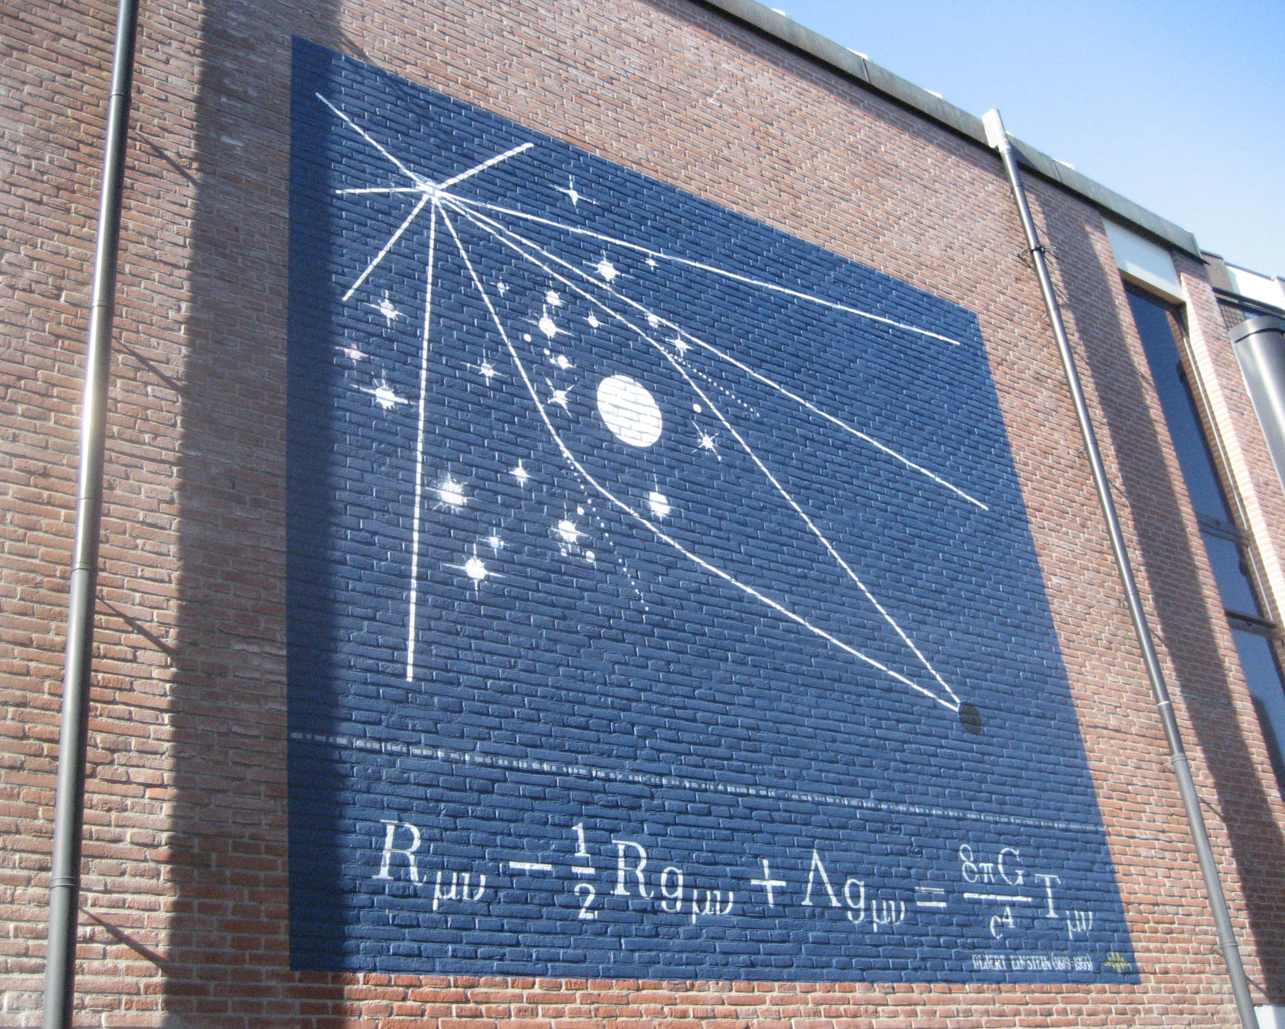
\includegraphics[width=0.7\linewidth]{example-fig}%[<选项>]{<figures目录下的文件名>
			\caption{这是一个示例图片}%图片的标题
			\label{fig:一个示例图片}%给图片一个标签方便交叉引用,\label必须放在\caption之后
		\end{figure}
	\end{latexcode}

	\begin{figure}[htbp]%或[H]
		\centering
		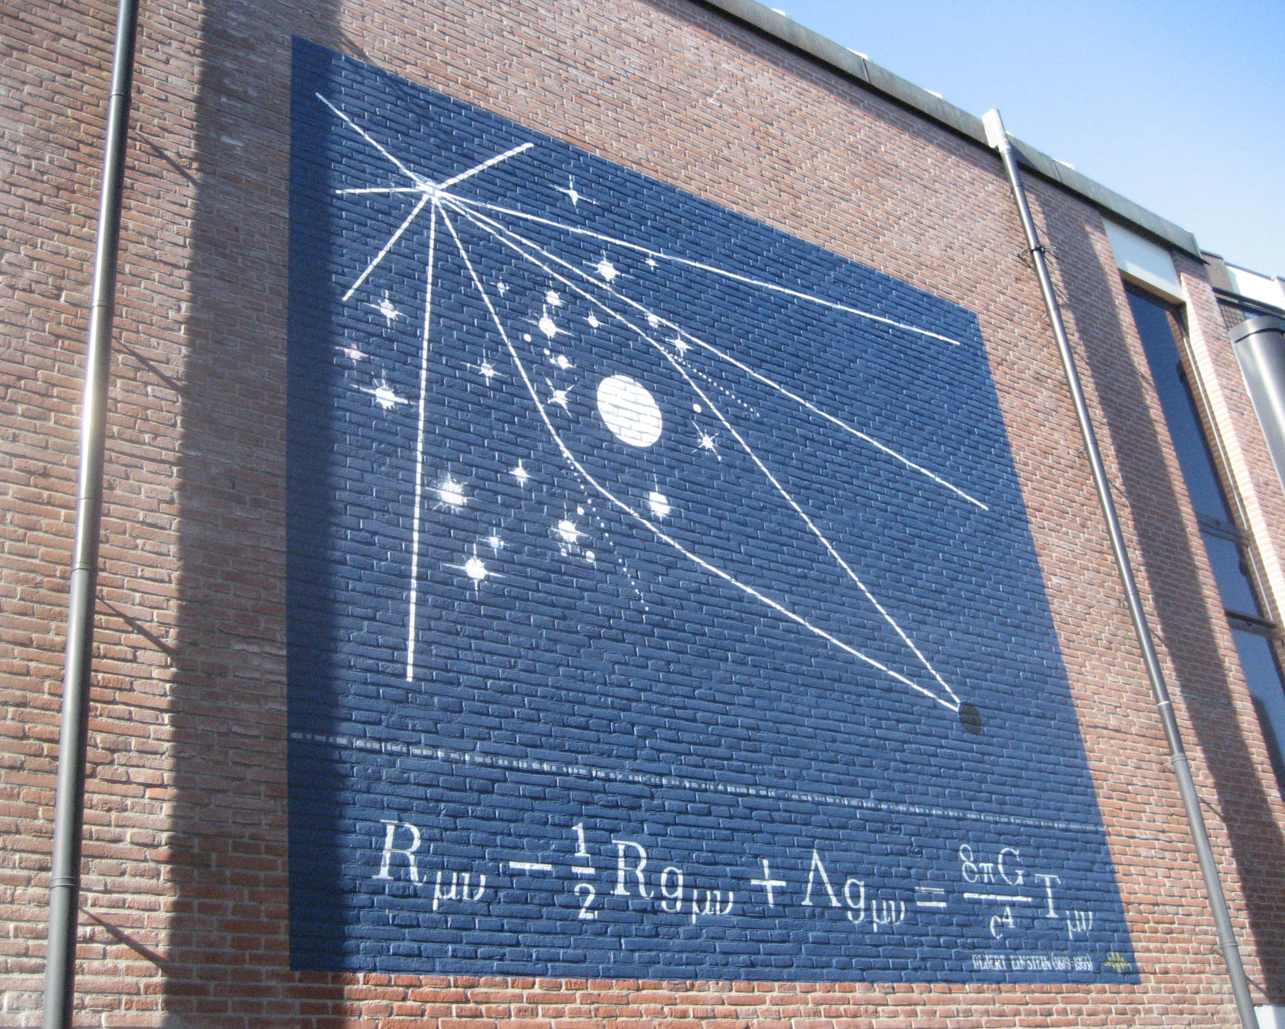
\includegraphics[width=0.7\linewidth]{example-fig}
		\caption{这是一个示例图片}
		\label{fig:一个示例图片}
	\end{figure}

	\begin{latexcode}
		引用图片,\autoref{fig:一个示例图片}。
	\end{latexcode}\textbf{编译得:}引用图片,\autoref{fig:一个示例图片}。

	此外,可选项可用width、height、scale、angle来设置图形的宽度、高度、缩放比例以及其逆时针旋转的角度,具体说明见\autoref{tab:includegraphics可选参数说明}。值得一提的是\lstinline[language=latex]|\linewidth|命令,它表示当前文本行的宽度,在不同环境中会有所不同。
	
	\begin{table}[htbp]
		\centering
		\caption{\textbackslash includegraphics命令常用可选参数说明\label{tab:includegraphics可选参数说明}}
		\begin{tabular}{cc}
			\toprule
			参数           &       含义 \\
			\midrule
			\verb|width|$=<width>$   &  设置图片宽度为$<width>$ \\
			\verb|height|$=<height>$ &  设置图片高度为$<height>$\\
			\verb|scale|$=<scale>$   &  将图片缩放为原来的$<scale>$倍 \\
			\verb|angle|$=<angle>$   &  将图片逆时针旋转$<angle>$度 \\
			\verb|origin=l/r/c/t/b/B|&  指明旋转中心(左/右/中/上/下/基线)  \\
			\bottomrule
		\end{tabular}
	\end{table}
	
	\newpage
	多图共用一个标题可使用如下代码:
	\begin{latexcode}
		\begin{figure}[H]
			\centering
			\begin{minipage}{\linewidth}
				\centering
				\includegraphics[width=.4\linewidth]{example-image-a}
				\includegraphics[width=.4\linewidth]{example-image-b}
			\end{minipage}\vspace{3pt}
			\begin{minipage}{\linewidth}
				\centering
				\includegraphics[width=.4\linewidth]{example-image-b}
				\includegraphics[width=.4\linewidth]{example-image-a}
			\end{minipage}
			\caption{多图共用一个标题\label{fig:多图共用一个标题}}
		\end{figure}
	\end{latexcode}
	
	\begin{figure}[H]
		\centering
		\begin{minipage}{\linewidth}
			\centering
			\includegraphics[width=.4\linewidth]{example-image-a}
			\includegraphics[width=.4\linewidth]{example-image-b}
		\end{minipage}\vspace{3pt}
		\begin{minipage}{\linewidth}
			\centering
			\includegraphics[width=.4\linewidth]{example-image-b}
			\includegraphics[width=.4\linewidth]{example-image-a}
		\end{minipage}
		\caption{多图共用一个标题\label{fig:多图共用一个标题}}
	\end{figure}

	\begin{latexcode}
		引用图片,\autoref{fig:多图共用一个标题}。
	\end{latexcode}\textbf{编译得:}引用图片,\autoref{fig:多图共用一个标题}。
	
	\newpage
	多图拥有各自的标题可使用如下代码:

	\begin{latexcode}
		\begin{figure}[H]
			\centering
			\begin{minipage}{.47\linewidth}
				\centering
				\includegraphics[width=\linewidth]{example-image-a}
				\caption{并排图1\label{fig:并排图1}}
			\end{minipage}\hspace{1em}%增加1em的水平间距
			\begin{minipage}{.47\linewidth}
				\centering
				\includegraphics[width=\linewidth]{example-image-b}
				\caption{并排图2\label{fig:并排图2}}
			\end{minipage}
		\end{figure}
	\end{latexcode}

	\begin{figure}[H]
		\centering
		\begin{minipage}{.47\linewidth}
			\centering
			\includegraphics[width=\linewidth]{example-image-a}
			\caption{并排图1\label{fig:并排图1}}
		\end{minipage}\hspace{1em}%增加1em的水平间距
		\begin{minipage}{.47\linewidth}
			\centering
			\includegraphics[width=\linewidth]{example-image-b}
			\caption{并排图2\label{fig:并排图2}}
		\end{minipage}
	\end{figure}

	\begin{latexcode}
		引用图片,\autoref{fig:并排图1}、\autoref{fig:并排图2}。
	\end{latexcode}\textbf{编译得:}引用图片,\autoref{fig:并排图1}、\autoref{fig:并排图2}。

	\newpage
	多图有各自的子标题,同时共用一个大标题可使用如下代码:
	
	\begin{latexcode}
		\begin{figure}[H]
			\centering
			\begin{subfigure}{.47\linewidth}
				\centering
				\includegraphics[width=\linewidth]{example-image-a}
				\subcaption{子图1\label{fig:子图1}}
			\end{subfigure}
			\hspace{1em}%增加1em的水平间距
			\begin{subfigure}{.47\linewidth}
				\centering
				\includegraphics[width=\linewidth]{example-image-b}
				\subcaption{子图2\label{fig:子图2}}
			\end{subfigure}
			\caption{并排插图的大标题\label{fig:并排插图的大标题}}
		\end{figure}
	\end{latexcode}
	
	\begin{figure}[H]
		\centering
		\begin{subfigure}{.47\linewidth}
			\centering
			\includegraphics[width=\linewidth]{example-image-a}
			\subcaption{子图1\label{fig:子图1}}
		\end{subfigure}
		\hspace{1em}%增加1em的水平间距
		\begin{subfigure}{.47\linewidth}
			\centering
			\includegraphics[width=\linewidth]{example-image-b}
			\subcaption{子图2\label{fig:子图2}}
		\end{subfigure}
		\caption{并排插图的大标题\label{fig:并排插图的大标题}}
	\end{figure}
	
	\begin{latexcode}
		引用图片,\autoref{fig:子图1}、\autoref{fig:子图2}及\autoref{fig:并排插图的大标题}。
	\end{latexcode}\textbf{编译得:}引用图片,\autoref{fig:子图1}、\autoref{fig:子图2}及\autoref{fig:并排插图的大标题}。
	
	最后要说的是,插图方式不固定,怎么好用怎么用!更多插图方式可参考\href{https://www.latexstudio.net/archives/8652.html}{\LaTeX 插图总结}。
	\subsubsection{使用TikZ绘图}
	\LaTeX 除了用来排版文字,还可用代码绘制图形,这里推荐一个绘图工具\href{https://github.com/csekri/tkzgeom}{GUI tool for TikZ figure production}。

	\subsection{画三线表}
	在研究过程中,通常将数据保存为\verb|.xlsx|或\verb|.csv|等格式,可通过\href{https://tableconvert.com/}{表格在线转换}将其转换为\LaTeX 代码。以下代码展示了一个三线表的例子。
	
	\begin{latexcode}
		\begin{table}[htbp]
			\centering
			\caption{An example Table.}
			\label{tab:example-tab}
			\begin{tabular}{lcc}
				\toprule
				Star & Mass & Luminosity\\
				& $M_{\odot}$ & $L_{\odot}$\\
				\midrule
				Sun & 1.00 & 1.00\\
				$\alpha$~Cen~A & 1.10 & 1.52\\
				$\epsilon$~Eri & 0.82 & 0.34\\
				\bottomrule
			\end{tabular}
		\end{table}
	\end{latexcode}

	\textbf{编译得:}
	\begin{table}[htbp]
		\centering
		\caption{An example Table.}
		\label{tab:example-tab}
		\begin{tabular}{lcc}
			\toprule
			Star & Mass & Luminosity\\
			& $M_{\odot}$ & $L_{\odot}$\\
			\midrule
			Sun & 1.00 & 1.00\\
			$\alpha$~Cen~A & 1.10 & 1.52\\
			$\epsilon$~Eri & 0.82 & 0.34\\
			\bottomrule
		\end{tabular}
	\end{table}

	\autoref{tab:example-tab} 的源代码中应注意:
	
	\begin{itemize}
		\item \lstinline[language=latex]|\label{}|必须置于\lstinline[language=latex]|\caption{}|之后;
		
		\item 表中每一列用\verb|&|分割,换行用\verb|\\|;
		
		\item \lstinline[language=latex]|\toprule|:画表格顶部粗线,其粗细可用\lstinline[language=latex]|\heavyrulewidth|设置;
		
		\item \lstinline[language=latex]|\midrule|:画表格中间分隔线,其粗细可用\lstinline[language=latex]|\lightrulewidth|设置;
		
		\item \lstinline[language=latex]|\bottomrule|:画表格底部粗线,其粗细可用\lstinline[language=latex]|\heavyrulewidth|设置;
		
		\item
		\lstinline[language=latex]|\cmidrule{<起>-<止>}|:画指定列的分隔线,其粗细可用\lstinline[language=latex]|\cmidrulewidth|设置。
	\end{itemize}

	\autoref{tab:example-tab} 的源代码中的\verb|lcc|表示:第一列左对齐,第二列居中对齐,第三列居中对齐。\autoref{tab:表格列格式说明}给出了\LaTeX 表格列格式的说明。
	
	\begin{table}[H]
		\centering
		\caption{\LaTeX 表格列格式说明}
		\label{tab:表格列格式说明}
		\begin{tabular}{>{\small}l>{\footnotesize}c}%列格式说明:两列,第一列左对齐,第二列居中齐,同时使用array宏包提供的>{<内容>}(表示把<内容>插入其后所在列的开头)设置各列字体尺寸
			\toprule %画表格顶部粗线
			\textbf{列格式} & \textbf{\small 说明} \\%第一列标题加粗,第二列标题在加粗的同时把字体尺寸设为small,然后用\\换行
			\midrule %画表格中间分隔线
			\verb|l|   &   本列左对齐   \\
			\verb|c|   &   本列居中   \\
			\verb|r|   &   本列右对齐   \\
			\verb|p{<宽度>}|   &   指定列宽   \\
			\verb|||   &   绘制竖线   \\
			\verb|@{<内容>}|   &   自定义内容   \\
			\verb|*{<计数>}{<列格式说明>}|     &     给出\verb|<列格式说明>|的重复次数   \\
			\bottomrule %画表格底部粗线
		\end{tabular}
	\end{table}

	\autoref{tab:表格列格式说明}的源代码为:
	\begin{latexcode}
		\begin{table}[htbp]
			\centering
			\caption{\LaTeX 表格列格式说明}
			\label{tab:表格列格式说明}
			\begin{tabular}{>{\small}l>{\footnotesize}c}%列格式说明:两列,第一列左对齐,第二列居中齐,同时使用array宏包提供的>{<内容>}(表示把<内容>插入其后所在列的开头)设置各列字体尺寸
				\toprule %画表格顶部粗线
				\textbf{列格式} & \textbf{\small 说明} \\%第一列标题加粗,第二列标题在加粗的同时把字体尺寸设为small,然后用\\换行
				\midrule %画表格中间分隔线
				\verb|l|   &   本列左对齐   \\
				\verb|c|   &   本列居中   \\
				\verb|r|   &   本列右对齐   \\
				\verb|p{<宽度>}|   &   指定列宽   \\
				\verb|||   &   绘制竖线   \\
				\verb|@{<内容>}|   &   自定义内容   \\
				\verb|*{<计数>}{<列格式说明>}|     &     给出\verb|<列格式说明>|的重复次数   \\
				\bottomrule %画表格底部粗线
			\end{tabular}
		\end{table}
	\end{latexcode}

	\subsection{罗列环境}
	无序列表:
	\begin{latexcode}
		\begin{itemize}
			\item 第一项。
			\item 第二项。
		\end{itemize}
	\end{latexcode}

	\textbf{编译得:}
	\begin{itemize}
		\item 第一项。
		\item 第二项。
	\end{itemize}
	
	有序列表:
	\begin{latexcode}
		\begin{enumerate}
			\item 第一项。
			\item 第二项。
		\end{enumerate}
	\end{latexcode}
	
	\textbf{编译得:}
	\begin{enumerate}
		\item 第一项。
		\item 第二项。
	\end{enumerate}

	\subsection{致谢部分}
	致谢部分使用如下代码撰写:
	\begin{latexcode}
		\begin{acknowledgement}
			致谢的内容。
		\end{acknowledgement}
	\end{latexcode}

	\subsection{文献引用}
	先在\href{https://oversea.cnki.net/}{知网}、\href{https://scholar.google.com/}{Google Scholar}和\href{https://ui.adsabs.harvard.edu/}{NASA/ADS}等论文搜索引擎中搜索文献,再在其期刊官网导出参考文献的BibTeX数据。下载BibTeX数据的方法大同小异,为了方便起见,以百度学术为例。先\href{https://xueshu.baidu.com/usercenter/paper/show?paperid=1w410c80b32s0jc0xj6h00709e628265}{搜索文献}
	\begin{figure}[H]
		\centering
		
\includegraphics[width=.8\linewidth]{bibtex-1}
	\end{figure}点击``引用''按钮。
	\begin{figure}[H]
		\centering
		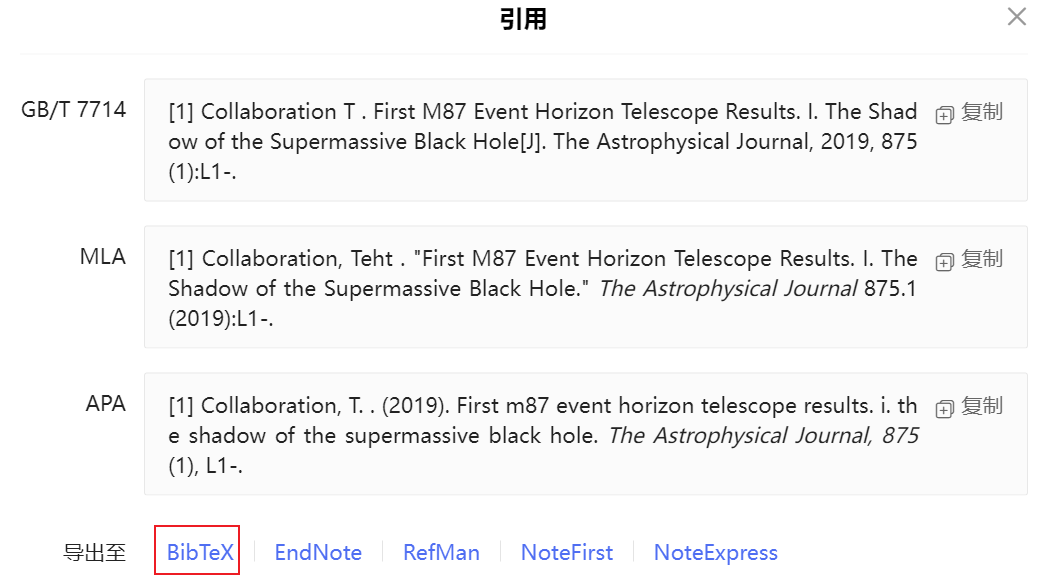
\includegraphics[width=.8\linewidth]{bibtex-2}
	\end{figure}点击``BibTeX''按钮。
	\begin{figure}[H]
		\centering
		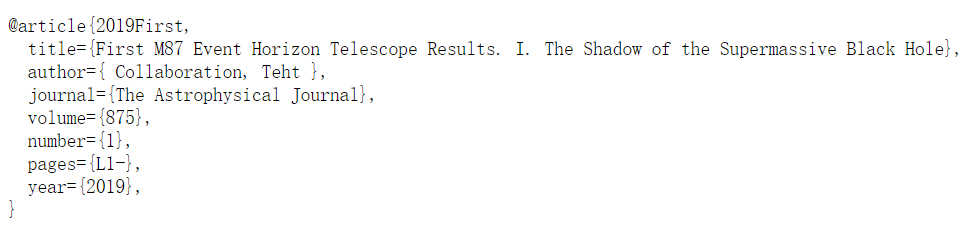
\includegraphics[width=.8\linewidth]{bibtex-3}
	\end{figure}将以上内容复制到\verb|references/references.bib|文件里。上图中的\verb|2019First|是一个标签,可修改为方便记忆的名称,便于引用文献。以下是引用文献的示例代码。若参考文献没有BibTeX数据或BibTeX数据不正确,请参照\href{https://github.com/zepinglee/gbt7714-bibtex-style/blob/master/test/testbst/support/standard.bib}{示例文件}填写。

	\begin{latexcode}
		引用\cite{2019First}。引用\cite{向守平2008天体物理概论}。引用\cite{BQC_2020}。引用\cite{2019First,向守平2008天体物理概论,BQC_2020}。
	\end{latexcode}
	\textbf{编译得:}引用\cite{2019First}。引用\cite{向守平2008天体物理概论}。引用\cite{BQC_2020}。引用\cite{2019First,向守平2008天体物理概论,BQC_2020}。
	
	\subsection{代码片段}
	插入代码片段可使用如下命令:
	\begin{latexcode}
		\lstset{style=codestyle}%全局设置一次codestyle即可
		\lstinputlisting[language=python]{code/Python example.py}
	\end{latexcode}

	\textbf{编译得:}
	{\lstset{style=codestyle}%设置一次codestyle即可
	\lstinputlisting[language=python]{code/Python example.py}}

	\subsection{附录}
	附录的示例代码如下:
	\begin{latexcode}
		\appendix
		\section{附录}
			\subsection{\LaTeX~Source Code}
				\lstinputlisting[language=latex,caption={\LaTeX~Source Code}]{main.tex}
			\subsection{Some Examples 2}
				some text...
	\end{latexcode}
	
	\section{编译文档}
	在命令行输入如下命令:
	\begin{itemize}
		\item 编译命令:\verb|latexmk|
		\item 清除编译过程中产生的辅助文件:\verb|latexmk -c|
	\end{itemize}若参考文献出现类似\verb|[?]|和目录未及时更新等情况,请先清除编译过程中产生的辅助文件,再执行编译命令。
	
	\section{PDF转Word}
	可使用 \href{https://www.adobe.com/acrobat/online/pdf-to-word.html}{Adobe PDF to Word} 转换 \verb|*.pdf| 文件。第二次转换文件时需要登录 Adobe 账号才能下载,建议在浏览器的“无痕浏览”、“隐私模式”等模式下访问以跳过强制登录。
	
	\begin{acknowledgement}
		致谢。
	\end{acknowledgement}

	\reference{references/references.bib}%参考文献,引入文献的bibtex格式信息,填bib文件
	
	\appendix
	\section{附录}
		\subsection{\LaTeX~Source Code}
			%\lstinputlisting[language=latex,caption={\LaTeX~Source Code}]{main.tex}
		\subsection{Some Examples 2}
			some text...

	\backcover%封底
\end{document}
